\documentclass{article}
\usepackage[utf8]{inputenc}
\usepackage{amsmath}
\usepackage{natbib}
\usepackage{graphicx}
\usepackage{listings}
\usepackage{color}
\usepackage{tikz}
\usepackage{multicol}
\usetikzlibrary{arrows}

\newcommand{\blank}[1]{\hspace*{#1}}
\newcommand{\answer}[1]{\underline{\underline{#1}}}

\definecolor{codegreen}{rgb}{0,0.6,0}
\definecolor{codegray}{rgb}{0.5,0.5,0.5}
\definecolor{codepurple}{rgb}{0.58,0,0.82}
\definecolor{backcolour}{rgb}{0.95,0.95,0.92}
 
\lstdefinestyle{mystyle}{
    backgroundcolor=\color{backcolour},   
    commentstyle=\color{codegreen},
    keywordstyle=\color{magenta},
    numberstyle=\tiny\color{codegray},
    stringstyle=\color{codepurple},
    basicstyle=\footnotesize,
    breakatwhitespace=false,         
    breaklines=true,                 
    captionpos=b,                    
    keepspaces=true,                 
    numbers=left,                    
    numbersep=5pt,                  
    showspaces=false,                
    showstringspaces=false,
    showtabs=false,                  
    tabsize=2
}
 
\lstset{style=mystyle}
\lstset{
    language=Erlang,
    mathescape=true
}

\title{MEK1100 - Oblig 1}
\author{Hans-Petter Harveg}
\date{Februar 2018}

\begin{document}

\maketitle

%
% PROBLEM:
%

\section*{Oppgaver}


\bigskip

\subsection*{Oppgave 1}

%
% a):
%

\subsection*{a)}

\begin{flushleft}
Vi har at:
\end{flushleft}

\begin{equation*}
x(t) = v_0 t \cos{\theta}
\end{equation*}
\begin{equation*}
y(t) = v_0 t \sin{\theta} - \frac{1}{2}g t^2
\end{equation*}

\begin{flushleft}
Og skal finne \(t_m\) og \(x_m\):
\end{flushleft}

\begin{align*}
v_0 t \sin{\theta} - \frac{1}{2}gt^2 = 0
\end{align*}

\begin{align*}
t(v_0 \sin{\theta} - \frac{1}{2}gt) = 0
\end{align*}

\begin{flushleft}
Så får vi at:
\end{flushleft}

\begin{center}
\(t = 0\) \ \ \ og \ \ \ \(v_0 \sin{\theta} - \frac{1}{2}gt = 0\)
\end{center}

\bigskip

\begin{flushleft}
Som da er tiden i start og stop. Løser vi så for \(t\) får vi:
\end{flushleft}

\begin{align*}
\frac{1}{2}gt  = v_0\sin{\theta}
\end{align*}

\begin{align*}
t_m  = \frac{2v_0\sin{\theta}}{g}
\end{align*}

\bigskip

\begin{flushleft}
Dette setter vi inn i \(x\) som gir oss:
\end{flushleft}

\begin{align*}
x_m & = x(t_m) \\ \\
 & = v_0(\frac{2v_0\sin{\theta}}{g})\cos{\theta} \\ \\
 & = \frac{2v_0^2\sin{\theta}\cos{\theta}}{g} \\ \\
 & = \frac{v_0^2\sin{2\theta}}{g}
\end{align*}

%
% b):
%

\subsection*{b)}

\begin{flushleft}
Vi skal så inføre dimensjonsløse variable. I og med at det ikke står noe om høyden går jeg ut fra at vi også her skal bruke \(x_m\).
\end{flushleft}

\begin{multicols}{2}
\begin{align*}
x^* & = \frac{x}{x_m} \\ \\
 & = \frac{v_0 t \cos{\theta}}{\frac{2v_0^2\sin{\theta}\cos{\theta}}{g}} \\ \\
 & = \frac{v_0 t \cos{\theta} g}{2v_0^2\sin{\theta}\cos{\theta}} \\ \\
 & = \frac{gt}{2v_0\sin{\theta}}
\end{align*}

\begin{align*}
t^* & = \frac{t}{t_m} \\ \\
 & = \frac{t}{\frac{2v_0\sin{\theta}}{g}} \\ \\
 & = \frac{gt}{2v_0\sin{\theta}} \\ \\
 & = x^*
\end{align*}
\end{multicols}

\begin{flushleft}
Vi ser at \(t^* = x^*\).
\end{flushleft}

\begin{flushleft}
For \(y^*\) får vi:
\end{flushleft}

\begin{align*}
y^* & = \frac{y}{x_m} = \frac{v_0t\sin{\theta} - \frac{1}{2}gt^2}{\frac{v_0^{2}2\sin{\theta}\cos{\theta}}{g}} \\ \\
 & = \frac{v_0t\sin{\theta}}{\frac{v_0^{2}2\sin{\theta}\cos{\theta}}{g}} - \frac{\frac{1}{2}gt^2}{\frac{v_0^{2}2\sin{\theta}\cos{\theta}}{g}} \\ \\
 & = \frac{v_{0}x^*\sin{\theta}}{v_{0}\cos{\theta}} - \frac{\frac{1}{2}g t x^*}{v_0\cos{\theta}} \\ \\
 & = x^*\tan{\theta} - \frac{g t x^*}{2 v_{0}\cos{\theta}} \\ \\
 & = x^*\tan{\theta} - \frac{x^*2 v_{0}\sin{\theta}x^*}{2 v_{0}\cos{\theta}} \\ \\
 & = x^*\tan{\theta} - x^{*2}\tan{\theta} \\ \\
 & = (x^* - x^{*2})\tan{\theta}
\end{align*}

\bigskip

\begin{flushleft}
Grunnen til at vi ikke trenger å skalere vinkelen \(\theta\) er fordi det er et forholdstall og alt skalert for alle størrelser.
\end{flushleft}


%
% c):
%

\subsection*{c)}

\begin{flushleft}
I denne oppgaven har jeg skrevet en MATLAB-funksjon.
\end{flushleft}

\begin{lstlisting}[language=Matlab]
function[x, y] = Problem1c(a, b, theta)
    x = linspace(a, b, 100);
    y = (x - x.^2)*tan(theta);
end
\end{lstlisting}

\begin{lstlisting}[language=Matlab]
% Plot 1:
[x, y] = Problem1c(0, 1, pi/6);
plot(x, y, '-r');

hold on

% Plot 2:
[x, y] = Problem1c(0, 1, pi/4);
plot(x, y, '-m');

hold on

% Plot 3:
[x, y] = Problem1c(0, 1, pi/3);
plt = plot(x, y, '-b');

% Setup plot window:
legend('\pi/6','\pi/4','\pi/3');
xlabel('x');
ylabel('y');

axis([0 1, 0, 0.5]);
\end{lstlisting}

\bigskip

Plottet til dette scriptet ser ut som følger:

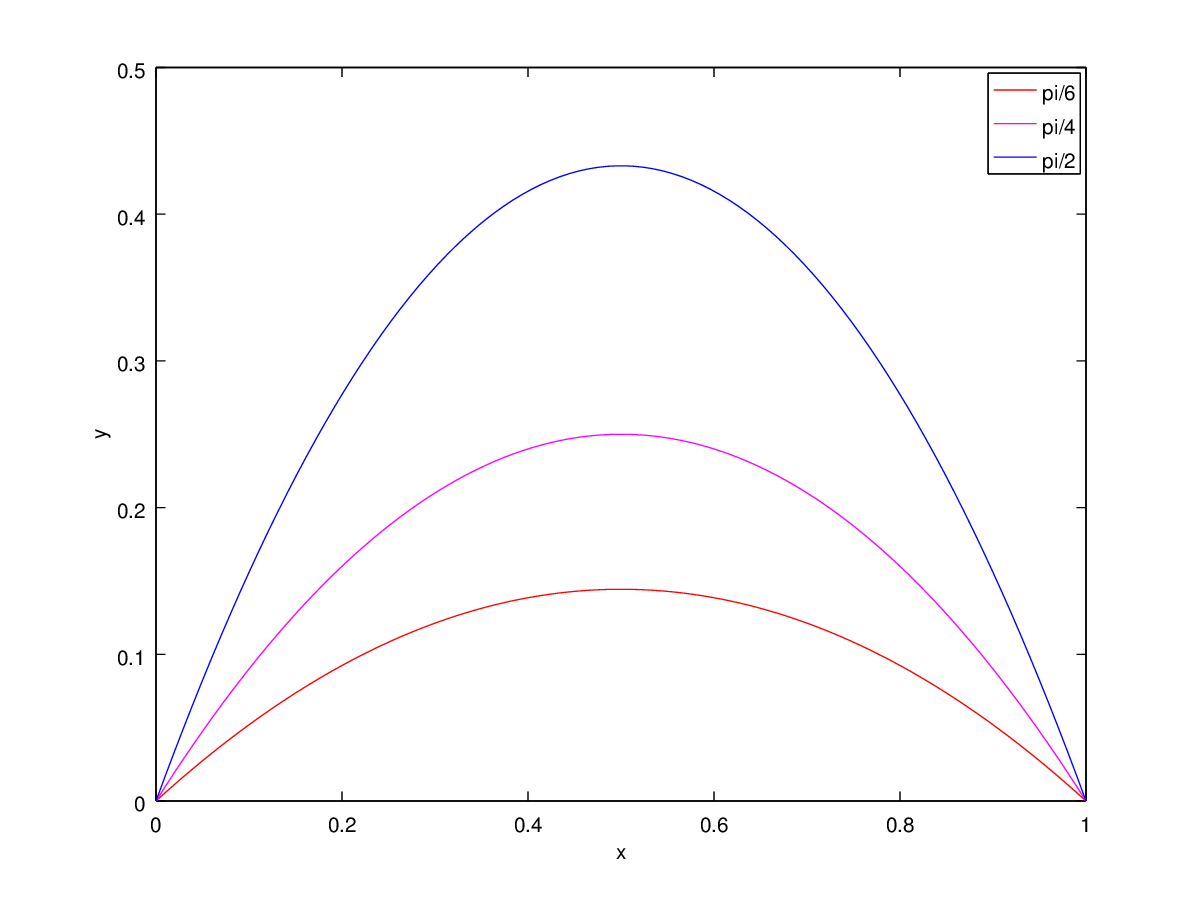
\includegraphics[scale=0.6]{images/Problem1c}

\newpage


%
% OPPGAVE 2
%

\section*{Oppgave 2}

%
% a)
%

\subsection*{a)}

\begin{flushleft}
Om vi betegner et vektorelement i tangetretning av strømlinjen med \(d\vec{r} = dx\vec{i} + dy\vec{j}\) må vektorene \(d\vec{r}\) og\(\vec{v}\) være parallelle og kan uttrykkes ved:
\end{flushleft}

\begin{equation*}
\vec{v} \times d\vec{r} = 0
\end{equation*}

\begin{flushleft}
Av dette får vi:
\end{flushleft}

\begin{align*}
\vec{v} \times d\vec{r} = \begin{bmatrix}
\vec{i} & \vec{j} & \vec{k} \\ v_x & v_y & 0 \\ dx & dy & 0 \end{bmatrix} 
 = \begin{vmatrix}v_y & 0 \\ dy & 0\end{vmatrix}\vec{i} - 
 \begin{vmatrix}v_x & 0 \\ v_x & 0\end{vmatrix}\vec{j} + 
 \begin{vmatrix}v_x & v_y \\ dx & dy\end{vmatrix}\vec{k} = (v_xdy - v_ydx)\vec{k} = 0
\end{align*}

\bigskip

\begin{flushleft}
Som viser at vi kan skrive:
\end{flushleft}

\begin{equation*}
v_xdy = v_ydx
\end{equation*}

\begin{flushleft}
Og for vårt uttrykk får vi da:
\end{flushleft}

\begin{equation*}
xy \ dy = y \ dx
\end{equation*}

\begin{equation*}
\int dy = \int \frac{1}{x} \ dx
\end{equation*}

\begin{equation*}
y = \ln{x} + C
\end{equation*}

\begin{flushleft}
Som viser at \(x \neq 0 \)
\end{flushleft}

\bigskip

\begin{flushleft}
Ser vi på på komponenene til \(\vec{v} \times d\vec{r}\):
\end{flushleft}

\begin{equation*}
v_y \cdot 0 - 0 \cdot dy = 0
\end{equation*}
\begin{equation*}
v_x \cdot 0 - 0 \cdot dx = 0
\end{equation*}

\bigskip

\begin{flushleft}
Den første ligningen impliserer at \(y = 0\) eller \(y = konstant\). Den andre at \(x=0\), \(y = 0\) eller at \(y = konstant\). Når \(y=0\) får vi x-aksen som løsning.
\end{flushleft}

%
% b)
%

\subsection*{b)}

\begin{flushle}
Vi finner stagnasjonspunkter når \(\vec{v} = 0\). Fordi \(x = 0\) ikke kan være en løsning for \(y\), vil vi finne stagnasjonspunktene når \(y = 0\). Dette betyr at hele x-aksen er stagnasjonspunkter. Beklager for en \textit{særdeles} stygg tegning:
\end{flushleft}

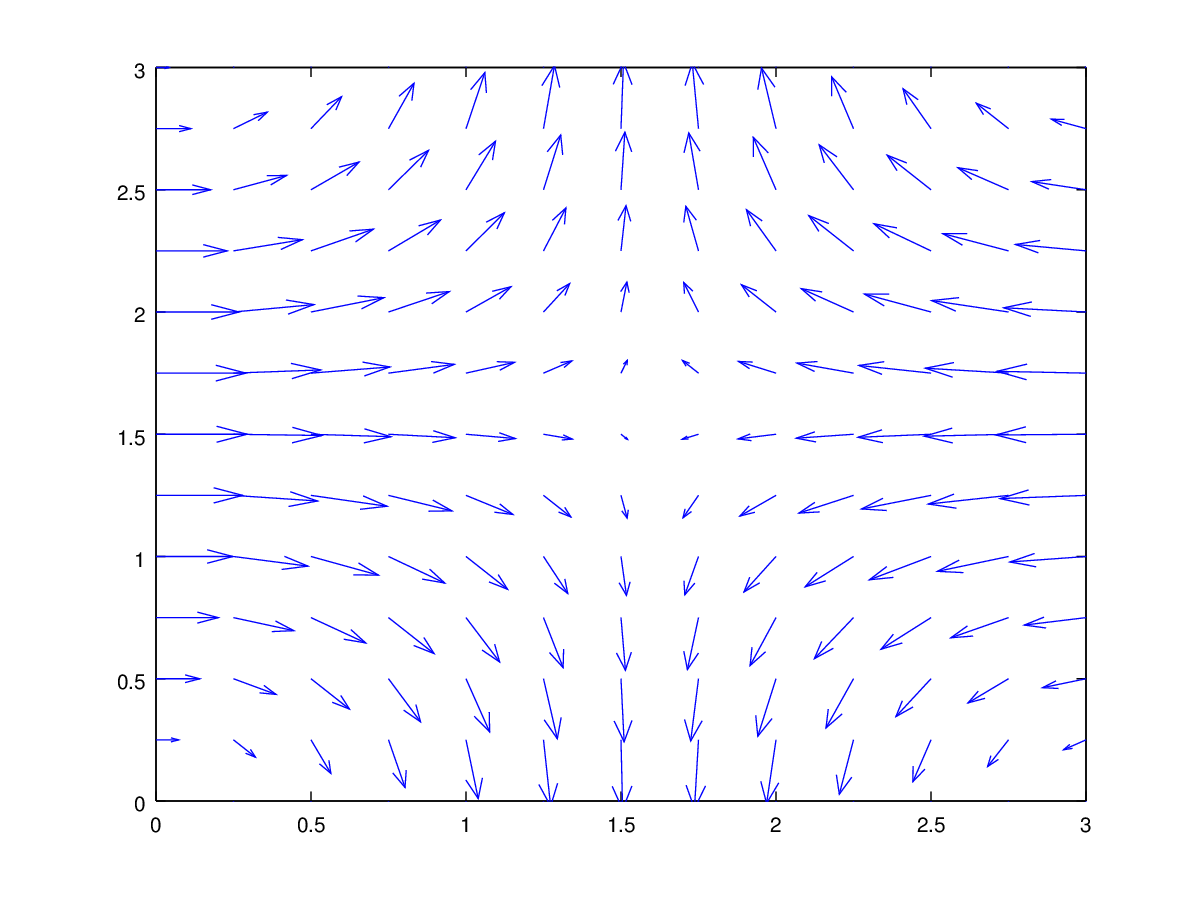
\includegraphics[scale=0.12]{images/Problem3b_streamlines}

\begin{flushleft}
Koden min ser ut som følger:
\end{flushleft}
\begin{lstlisting}[language=Matlab]
x = linspace(-5, 5, 10);
y = linspace(-5, 5, 10);

[x, y] = meshgrid(x,y);

u = x.*y;
v = y;

plt = figure;

quiver(x, y, u, v, 0.7);
hold on;

c = y - log(abs(x));

contour(x, y, c);

saveas(plt, 'Problem2b.png');
\end{lstlisting}

\newpage

\begin{flushleft}
Den gir plottet:
\end{flushleft}

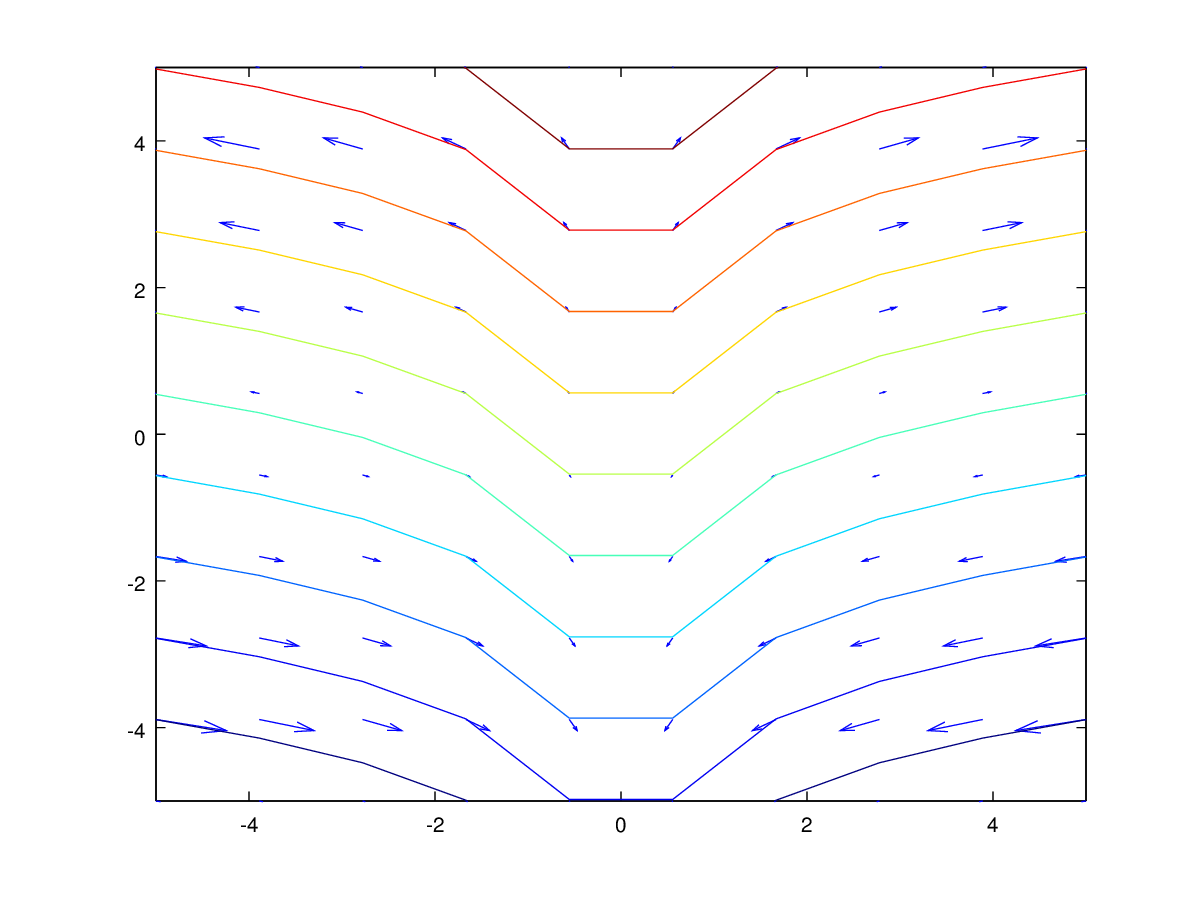
\includegraphics[scale=0.6]{images/Problem2b}

%
% c)
%

\subsection*{c)}

\begin{flushleft}
Strømfunksjonen \(\psi(x,y)\) har egenskapen at:
\end{flushleft}

\begin{equation*}
v_x = -\frac{\partial\psi}{\partial y} \ \ \ og \ \ \ v_y = \frac{\partial\psi}{\partial x} \end{equation*}

\begin{flushleft}
Vi får da:
\end{flushleft}

\begin{equation*}
\frac{\partial\psi}{\partial y} = -xy \ \ \ \Rightarrow \ \ \ \psi = -\frac{1}{2}xy^2 + g(x)
\end{equation*}

\begin{equation*}
\frac{\partial\psi}{\partial x} = y \ \ \ \Rightarrow \ \ \ \psi = xy + f(x)
\end{equation*}

\begin{flushleft}
Deriverer vi to ganger får vi:
\end{flushleft}

\begin{equation*}
\frac{\partial^2 \psi}{\partial x \partial y} = \frac{\partial}{\partial x}(\frac{\partial \psi}{\partial y}) = \frac{\partial}{\partial x}(-x y) = -y
\end{equation*}

\begin{equation*}
\frac{\partial^2\psi}{\partial x \partial y} = \frac{\partial}{\partial y}(\frac{\partial \psi}{\partial x}) = \frac{\partial}{\partial x}(y) = 1
\end{equation*}

\begin{flushleft}
Vi ser at de dobbelderiverte av \(\psi\) ikke er en konstant som betyr at det ikke finnes noen strømfunksjon.
\end{flushleft}


%
% OPPGAVE 3
%

\section*{Oppgave 3}

%
% a)
%

\subsection*{a)}

\begin{flushleft}
I denne oppgaven har vi at et hastighetsfelt i xy-planet git ved \vec{v} = u\vec{i} + v\vec{j} der:
\end{flushleft}

\begin{equation*}
u = \cos{x}\sin{y} \ \ \ og \ \ \ v = -\sin{x}\cos{y}
\end{equation*}

\bigskip

\begin{flushleft}
Divergens er definert ved:
\end{flushleft}

\begin{align*}
\nabla \cdot \vec{v} = \frac{\partial u}{\partial x} + \frac{\partial v}{\partial y}
\end{align*}

\begin{flushleft}
Vi har at:
\end{flushleft}
\begin{multicols}{2}
\begin{align*}
\frac{\partial u}{\partial x} = -\sin{x}\sin{y}
\end{align*}

\begin{align*}
\frac{\partial v}{\partial y} = \sin{x}\sin{y}
\end{align*}
\end{multicols}

\bigskip

\begin{flushleft}
Og får dermed:
\end{flushleft}

\begin{align*}
\nabla \cdot \vec{v} = \sin{x}\sin{y} - \sin{x}\sin{y} = \answer{0}
\end{align*}

\newpage


\begin{flushleft}
Vrivling er definert ved:
\end{flushleft}

\begin{align*}
\nabla \times \vec{u} & = \bigg( \frac{\partial u_3}{\partial y}- \frac{\partial u_2}{\partial z} , \frac{\partial u_1}{\partial z}- \frac{\partial u_3}{\partial x} , \frac{\partial u_2}{\partial x}- \frac{\partial u_1}{\partial y} \bigg)
\end{align*}

\begin{align*}
\begin{bmatrix}
\vec{i} & \vec{j} & \vec{k} \\
\frac{\partial}{\partial x} & \frac{\partial}{\partial y} & 0 \\ u & v & 0 \end{bmatrix} 
 = \begin{vmatrix}\frac{\partial}{\partial y} & 0 \\ v & 0\end{vmatrix}\vec{i} - 
 \begin{vmatrix}\frac{\partial}{\partial x} & 0 \\ u & v\end{vmatrix}\vec{j} + 
 \begin{vmatrix}\frac{\partial}{\partial x} & \frac{\partial}{\partial y} \\ u & v\end{vmatrix}\vec{k} = \bigg(\frac{\partial v}{\partial x} + \frac{\partial u}{\partial y} \bigg)\vec{k}
\end{align*}

\bigskip

\begin{flushleft}
Vi har at:
\end{flushleft}
\begin{multicols}{2}
\begin{align*}
\frac{\partial v}{\partial x} = -\cos{x}\cos{y}
\end{align*}

\begin{align*}
\frac{\partial u}{\partial y} = \cos{x}\cos{y}
\end{align*}
\end{multicols}

\bigskip

\begin{flushleft}
Og får dermed:
\end{flushleft}
\begin{align*}
\nabla \times \vec{v} = (-\cos{x}\cos{y} - \cos{x}\cos{y})\vec{k} = \answer{(-2\cos{x}\cos{y})\vec{k}}
\end{align*}

%
% b)
%

\subsection*{b)}

\begin{flushleft}
Vi har at:
\end{flushleft}
\begin{align*}
\vec{v}(x, y) & = v\vec{i} + v\vec{j} \\ \\
 & = \cos{x}\sin{y}\vec{i} + (-\sin{x}\cos{y})\vec{j} \\ \\
 & = \cos{x}\sin{y}\vec{i} - \sin{x}\cos{y}\vec{j}
\end{align*}
\begin{flushleft}
For x-aksen får vi:
\end{flushleft}
\begin{align*}
\vec{v}(x, 0) & = \cos{x}\sin{0}\vec{i} - \sin{x}\cos{0}\vec{j} \\ \\
 & = -\sin{x}\vec{j}
\end{align*}

\begin{flushleft}
For y-aksen får vi:
\end{flushleft}
\begin{align*}
\vec{v}(0, y) & = \cos{0}\sin{y}\vec{i} - \sin{0}\cos{y}\vec{j} \\ \\
 & = \sin{y}\vec{j}
\end{align*}

\bigskip

\begin{multicols}{2}
\begin{flushleft}
Størmvektorer langs x-aksen:
\end{flushleft}
\begin{flushleft}
Størmvektorer langs y-aksen:
\end{flushleft}
\end{multicols}

\begin{multicols}{2}
\begin{flushleft}
\(x = -1.5 \ \ \ \Rightarrow \ \ \ \vec{v} = 0.997\) \\
\(x = -1.0 \ \ \ \Rightarrow \ \ \ \vec{v} = 0.84\) \\
\(x = -0.5 \ \ \ \Rightarrow \ \ \ \vec{v} = 0.48\) \\
\(x = \ -0   \ \ \ \ \Rightarrow \ \ \ \vec{v} = 0\) \\
\(x = \ 0.5  \ \ \ \ \Rightarrow \ \ \ \vec{v} = -0.48\) \\
\(x = \ 1.0  \ \ \ \ \Rightarrow \ \ \ \vec{v} = -0.84\) \\
\(x = \ 1.5  \ \ \ \ \Rightarrow \ \ \ \vec{v} = -0.997\) \\
\end{flushleft}
\begin{flushleft}
\(y = -1.5 \ \ \ \Rightarrow \ \ \ \vec{v} = -0.997\) \\
\(y = -1.0 \ \ \ \Rightarrow \ \ \ \vec{v} = -0.84\) \\
\(y = -0.5 \ \ \ \Rightarrow \ \ \ \vec{v} = -0.48\) \\
\(y = \ -0   \ \ \ \ \Rightarrow \ \ \ \vec{v} = 0\) \\
\(y = \ 0.5  \ \ \ \ \Rightarrow \ \ \ \vec{v} = 0.48\) \\
\(y = \ 1.0  \ \ \ \ \Rightarrow \ \ \ \vec{v} = 0.84\) \\
\(y = \ 1.5  \ \ \ \ \Rightarrow \ \ \ \vec{v} = 0.997\) \\
\end{flushleft}
\end{multicols}

\begin{center}
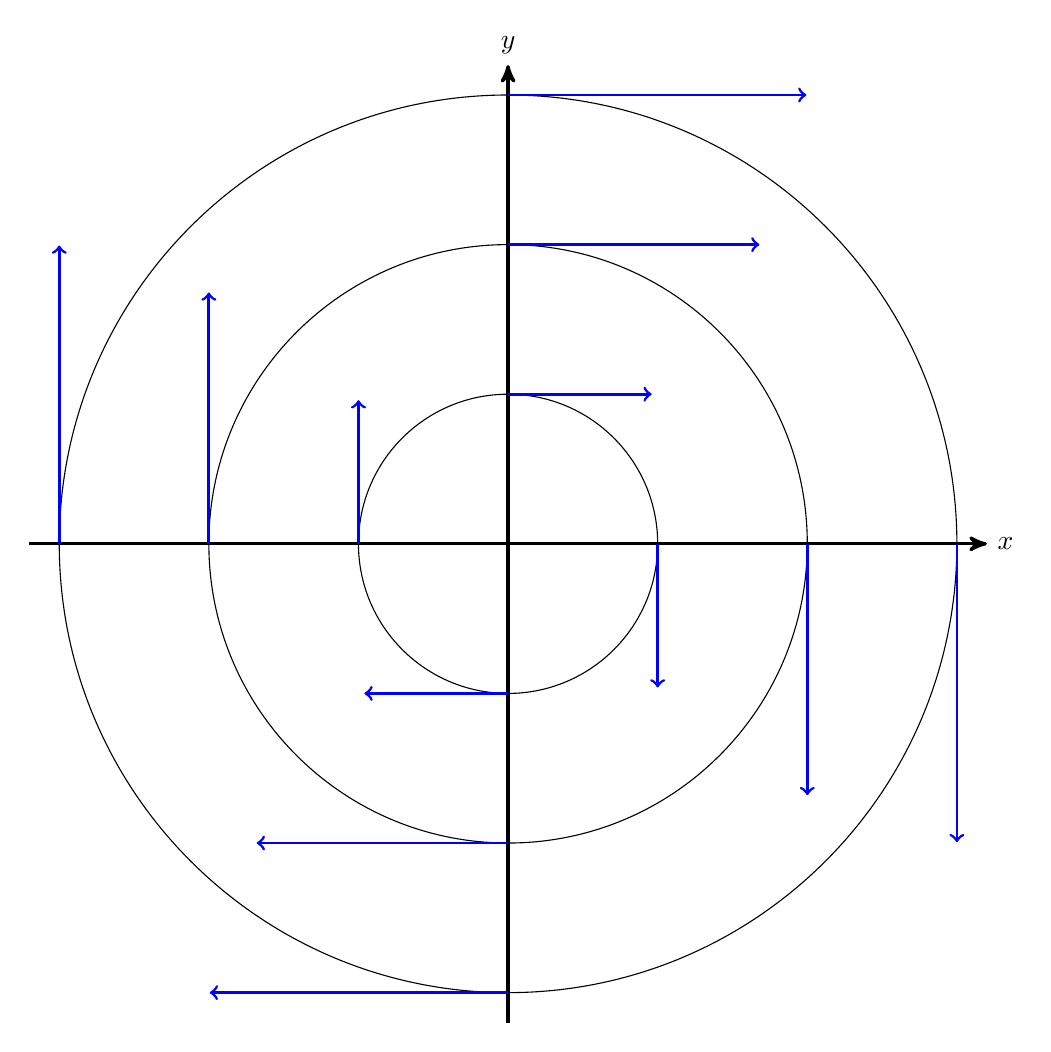
\begin{tikzpicture}[
    scale=3.8,
    axis/.style={very thick, ->, >=stealth'},
    important line/.style={thick},
    dashed line/.style={dashed, thin},
    pile/.style={thick, ->, >=stealth', shorten <=2pt, shorten
    >=2pt},
    every node/.style={color=black}
    ]
    
    % axis
    \draw[axis] (-1.6, 0)--(1.6, 0) node(xline)[right] {$x$};
    \draw[axis] (0,-1.6)--(0 ,1.6) node(yline)[above] {$y$};

    % 
    \draw (0.0, 0.0) circle (0.5);
    \draw (0.0, 0.0) circle (1.0);
    \draw (0.0, 0.0) circle (1.5);

    \draw[arrows=->,line width=1pt, color=blue!100] (0.0, 1.5)--(0.997, 1.5);
    \draw[arrows=->,line width=1pt, color=blue!100] (0.0, 1.0)--(0.84, 1.0);
    \draw[arrows=->,line width=1pt, color=blue!100] (0.0, 0.5)--(0.48, 0.5);
    
    \draw[arrows=->,line width=1pt, color=blue!100] (0.0, -1.5)--(-0.997, -1.5);
    \draw[arrows=->,line width=1pt, color=blue!100] (0.0, -1.0)--(-0.84, -1.0);
    \draw[arrows=->,line width=1pt, color=blue!100] (0.0, -0.5)--(-0.48, -0.5);
    
    \draw[arrows=->,line width=1pt, color=blue!100] (1.5, 0.0)--(1.5, -0.997);
    \draw[arrows=->,line width=1pt, color=blue!100] (1.0, 0.0)--(1.0, -0.84);
    \draw[arrows=->,line width=1pt, color=blue!100] (0.5, 0.0)--(0.5, -0.48);
    
    \draw[arrows=->,line width=1pt, color=blue!100] (-1.5, 0.0)--(-1.5, 0.997);
    \draw[arrows=->,line width=1pt, color=blue!100] (-1.0, 0.0)--(-1.0, 0.84);
    \draw[arrows=->,line width=1pt, color=blue!100] (-0.5, 0.0)--(-0.5, 0.48);

\end{tikzpicture}
\end{center}

\newpage

%
% c)
%

\subsection*{c)}

\begin{flushleft}
Vi funner sirkulasjonen om randa ved linjeintegralene til kvadratet. Vi kan dele opp i fire sider og regne de ut integralene hver for seg for så å legge de sammen:
\end{flushleft}

\begin{multicols}{2}
\begin{align*}
i_1 & = \int_{-\frac{\pi}{2}}^{\frac{\pi}{2}}\vec{v}\bigg(x, -\frac{\pi}{2}\bigg) \ dx \\ \\
 & = \int_{-\frac{\pi}{2}}^{\frac{\pi}{2}} \cos{(x)}\sin{(-\frac{\pi}{2})} \ dx \\ \\
 & = -\int_{-\frac{\pi}{2}}^{\frac{\pi}{2}} \cos{(x)} \ dx \\ \\
 & = -\bigg[ \sin{(x)} \bigg]_{-\frac{\pi}{2}}^{\frac{\pi}{2}} \\ \\
 & = -\bigg[ \sin{(\frac{\pi}{2})} - \sin{(-\frac{\pi}{2})} \bigg] \\ \\
 & = -\bigg[ 1-(-1) \bigg] \\ \\
 & = -2
\end{align*}

\begin{align*}
i_2 & = \int_{\frac{\pi}{2}}^{-\frac{\pi}{2}}\vec{v}\bigg(x, \frac{\pi}{2}\bigg) \ dx \\ \\
 & = \int_{\frac{\pi}{2}}^{-\frac{\pi}{2}} \cos{(x)}\sin{(\frac{\pi}{2})} \ dx \\ \\
 & = \int_{\frac{\pi}{2}}^{-\frac{\pi}{2}} \cos{(x)} \ dx \\ \\
 & = \bigg[ \sin{(x)} \bigg]_{\frac{\pi}{2}}^{-\frac{\pi}{2}} \\ \\
 & = \bigg[ \sin{(-\frac{\pi}{2})} - \sin{(\frac{\pi}{2})} \bigg] \\ \\
 & = \bigg[ -1-1 \bigg] \\ \\
 & = -2
\end{align*}
\end{multicols}

\newpage

\begin{multicols}{2}
\begin{align*}
j_1 & = \int_{-\frac{\pi}{2}}^{\frac{\pi}{2}}\vec{v}\bigg(\frac{\pi}{2}, y\bigg) \ dy \\ \\
 & = \int_{-\frac{\pi}{2}}^{\frac{\pi}{2}} (-\sin{(\frac{\pi}{2})}\cos{(y)}) \ dy \\ \\
 & = -\int_{-\frac{\pi}{2}}^{\frac{\pi}{2}} \cos{(y)} \ dy \\ \\
 & = -\bigg[ \sin{(y)} \bigg]_{-\frac{\pi}{2}}^{\frac{\pi}{2}} \\ \\
 & = -\bigg[ \sin{(\frac{\pi}{2})} - \sin{(-\frac{\pi}{2})} \bigg] \\ \\
 & = -\bigg[ 1-(-1) \bigg] \\ \\
 & = -2
\end{align*}

\begin{align*}
j_2 & = \int_{\frac{\pi}{2}}^{-\frac{\pi}{2}}\vec{v}\bigg(-\frac{\pi}{2}, y\bigg) \ dy \\ \\
 & = \int_{\frac{\pi}{2}}^{-\frac{\pi}{2}} (-\sin{(-\frac{\pi}{2})}\cos{(y)}) \ dy \\ \\
 & = \int_{\frac{\pi}{2}}^{-\frac{\pi}{2}} \cos{(y)} \ dy \\ \\
 & = \bigg[ \sin{(y)} \bigg]_{\frac{\pi}{2}}^{-\frac{\pi}{2}} \\ \\
 & = \bigg[ \sin{(-\frac{\pi}{2})} - \sin{(\frac{\pi}{2})} \bigg] \\ \\
 & = \bigg[ -1-1 \bigg] \\ \\
 & = -2
\end{align*}
\end{multicols}

\bigskip

\begin{flushleft}
Dermed får vi at sirkulasjonen om randa blir:
\end{flushleft}

\begin{equation*}
i_1 + i_2 + j_1 + j_2 = -2 + (-2) + (-2) + (-2) = \answer{-8}
\end{equation*}

\newpage

%
% d)
%

\subsection*{d)}

\begin{flushleft}
Fra a) vet vi at \(\nabla \cdot \vec{v} = 0\) som betyr at det eksisterer en strømfunksjon \(\psi(x,y)\)
\end{flushleft}

\begin{flushleft}
Vi har at:
\end{flushleft}

\begin{equation*}
u = -\frac{\partial \psi}{\partial y} \Rightarrow \frac{\partial \psi}{\partial y} = -u = -\cos{(x)}\sin{(y)} \Rightarrow \psi = \cos{(x)}\cos{(y)} + f(x)
\end{equation*}

\begin{equation*}
v = \frac{\partial \psi}{\partial x} \Rightarrow \frac{\partial \psi}{\partial x} = v = -\sin{(x)}\cos{(y)} \Rightarrow \psi = \cos{(x)}\cos{(y)} + g(y)
\end{equation*}

\bigskip

\begin{flushleft}
For å få en entydig løsning på \(\psi\) må \(f(x) = g(y) = 0\) og dermed er:
\end{flushleft}

\begin{equation*}
\psi = \cos{(x)}\cos{(y)}
\end{equation*}


%
% e)
%

\subsection*{e)}

\begin{flushleft}
Først regner vi ut de paritielderiverte til \(\psi\):
\end{flushleft}

\begin{equation*}
\frac{\partial \psi}{\partial x} = -\sin{(x)}\cos{(y)} \ \ \ \ \ \frac{\partial \psi}{\partial y} = -\cos{x}\sin{y}
\end{equation*}

\bigskip

\begin{equation*}
\frac{\partial^2 \psi}{\partial x^2} = -\cos{x}\cos{y} \ \ \ \ \ \frac{\partial^2 \psi}{\partial y^2} = -\cos{x}\cos{y}
\end{equation*}

\bigskip

\begin{equation*}
\frac{\partial^2 \psi}{\partial x\partial y} = \sin{x}\sin{y}
\end{equation*}

\bigskip

\begin{flushleft}
Taylorutviklingen av annen orden for \(\psi\) er definert ved:
\end{flushleft}

\begin{align*}
\psi(x, y)_{(0,0)} \approx \psi(0,0) + \bigg( \frac{\partial \psi}{ \partial x} \bigg)_{0,0}(x - 0) + \bigg( \frac{\partial \psi}{ \partial y} \bigg)_{0,0}(y - 0)
\end{align*}

\begin{align*}
+ \frac{1}{2}\bigg( \frac{\partial^2 \psi}{\partial x^2} \bigg)_{0,0}(x - 0)^2 + \frac{1}{2}\bigg( \frac{\partial^2 \psi}{\partial y^2} \bigg)_{0,0}(y - 0)^2
\end{align*}

\begin{align*}
+ \bigg( \frac{\partial^2 \psi}{\partial x \partial y} \bigg)_{0,0}(x - 0)(y - 0)
\end{align*}

\begin{flushleft}
Vi får da:
\end{flushleft}

\begin{align*}
= \cos{(0)}\cos{(0)} + (-\sin{(0)}\cos{(0)})x + (-\cos{(0)}\sin{(0)})y
\end{align*}
\begin{align*}
+ \frac{1}{2}(-\cos{(0)}\cos{(0)})x^2 + \frac{1}{2}(-\cos{(0)}\cos{(0)})y^2
\end{align*}
\begin{align*}
+ \sin{(0)}\sin{(0)}xy
\end{align*}

\begin{flushleft}
Som blir:
\end{flushleft}

\begin{align*}
1 + 0 + 0 + \frac{1}{2}(-1)x^2 + \frac{1}{2}(-1)y^2 + 0
\end{align*}

\begin{align*}
= \answer{1 - \frac{1}{2}x^2 - \frac{1}{2}y^2}
\end{align*}

\newpage

\section*{Oppgave 4}

%
% a)
%

\subsection*{a)}


\begin{lstlisting}[language=Matlab]
for n=[5 30]
    [x, y, psi] = streamfun(n);
    plt = figure;
    contour(x, y, psi);
    title(sprintf('Antall punkter: %d', n));
    saveas(plt, sprintf('Problem4a_%d.png', n));
end
\end{lstlisting}

\begin{flushleft}
Plottene vi får for henholdsvis \(n=5\) og \(n=30\) ser ut som følger:
\end{flushleft}

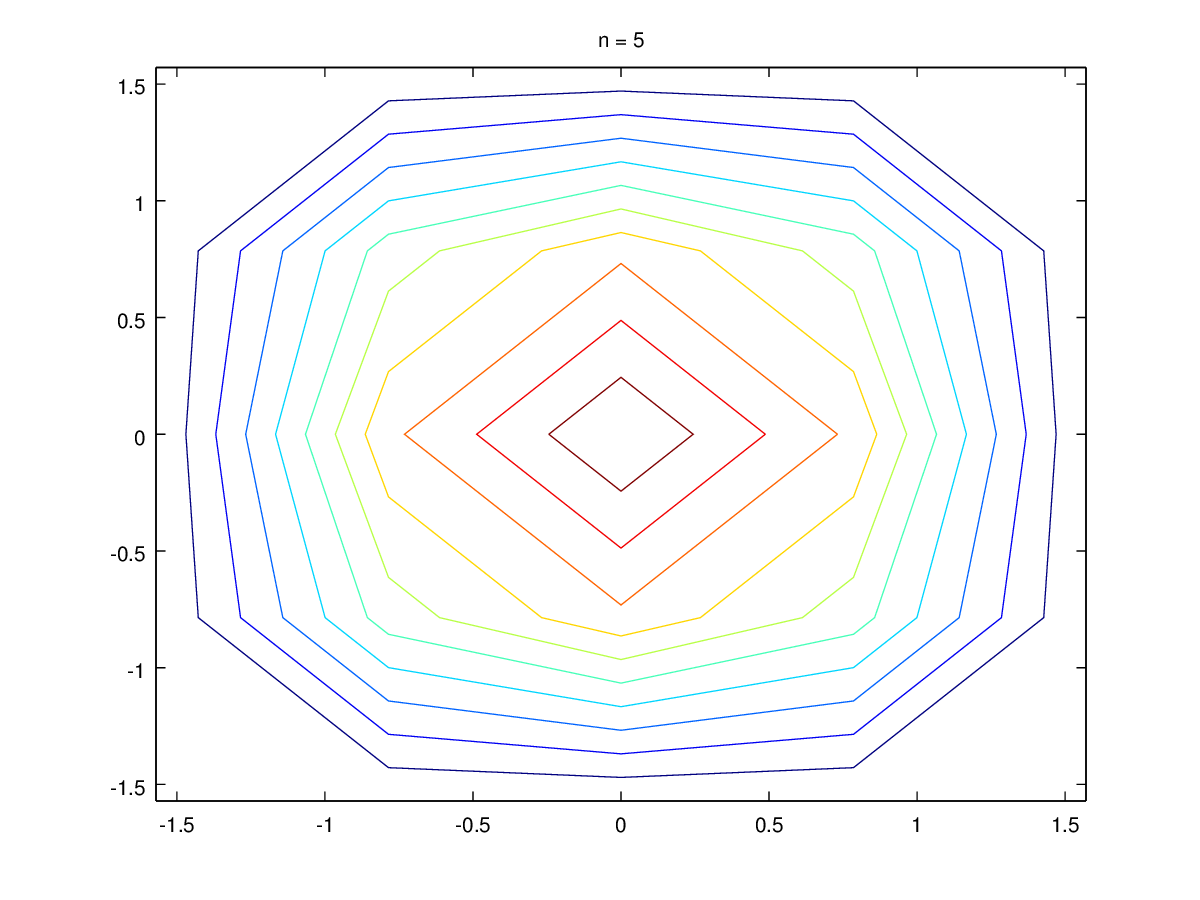
\includegraphics[scale=0.6]{images/Problem4a_5}

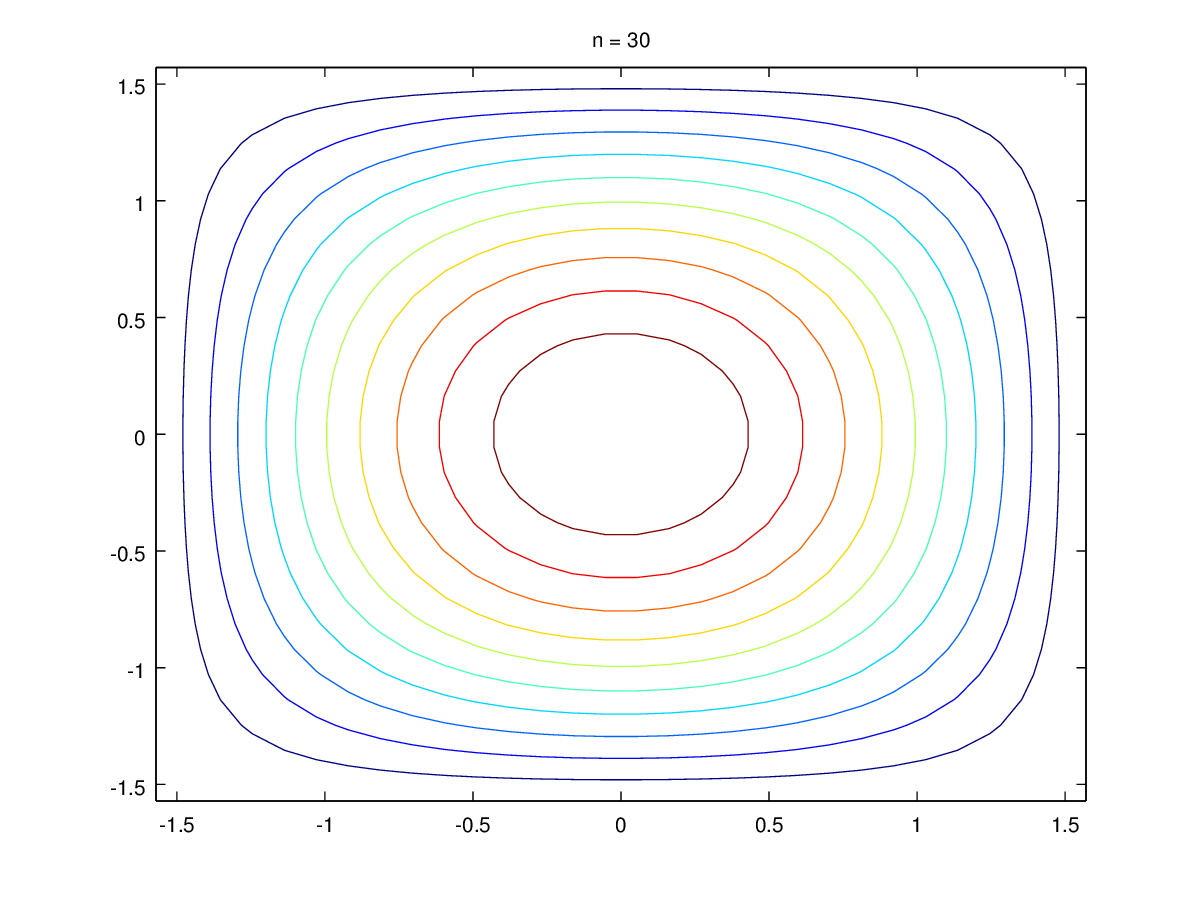
\includegraphics[scale=0.6]{images/Problem4a_30}

%
% b)
%

\subsection*{b)}

\begin{flushleft}
velfield-funksjonen ser ut som følger:
\end{flushleft}
\begin{lstlisting}[language=Matlab]
function [x, y, u, v] = velfield(n)

if nargin < 1;
    n=15;
end

x = linspace(-0.5*pi, 0.5*pi, n);

[x,y] = meshgrid(x,x);

u = cos(x).*sin(y);
v = -sin(x).*cos(y)
\end{lstlisting}

\begin{flushleft}
Vi kan bruke den på følgende måte:
\end{flushleft}
\begin{lstlisting}[language=Matlab]
n = 20;
[x,y,u,v] = velfield(n);
plt = figure;
quiver(x,y,u,v);
saveas(plt, sprintf('Problem4b_%d.png', n));
\end{lstlisting}

\begin{flushleft}
Plottet for \(n = 15\) vil da se ut som følger:
\end{flushleft}

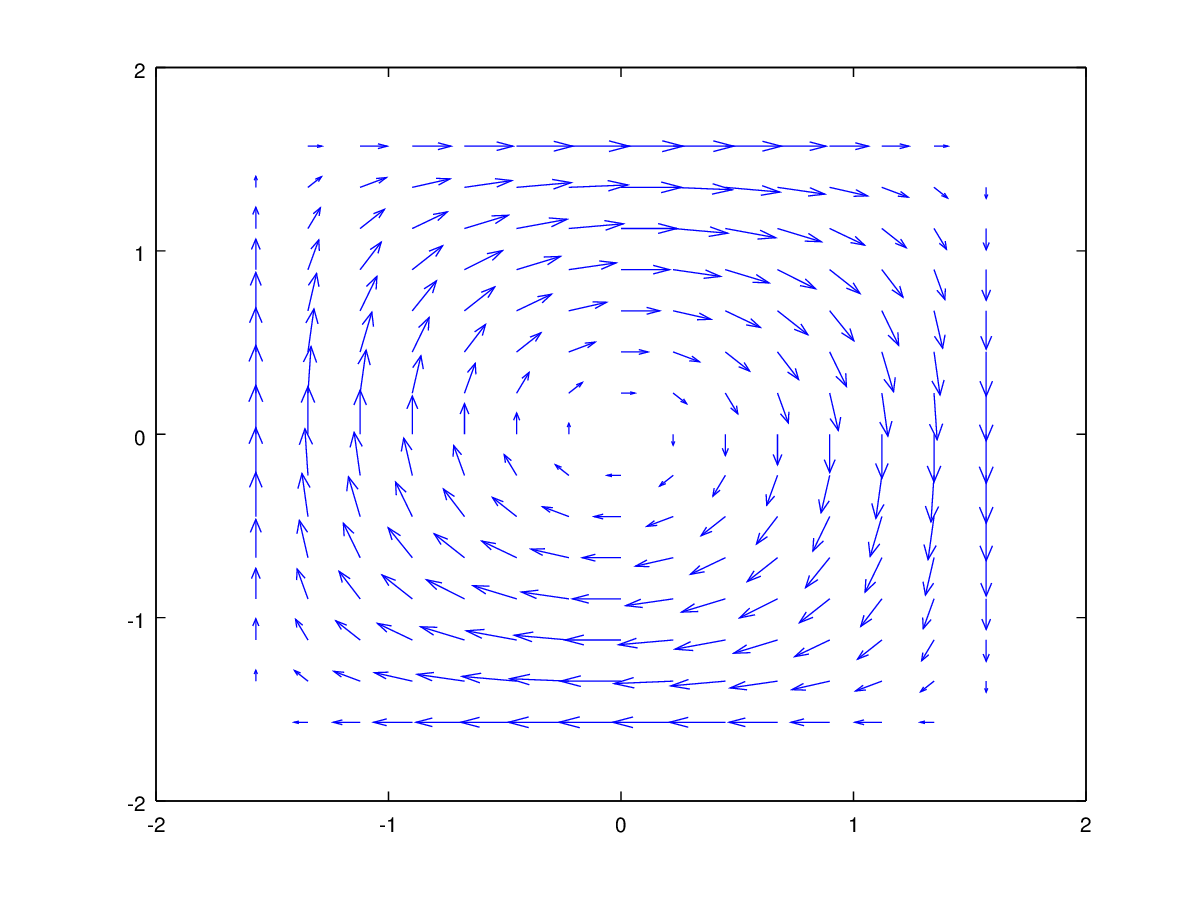
\includegraphics[scale=0.6]{images/Problem4b_15}


\bigskip

\bigskip

\bigskip

\bigskip


\begin{center}
\textit{Bazinga!}
\end{center}

\end{document}

